%!TEX root = ../main.tex



\section{sommario}

\begin{itemize}



 



    \item \textbf{Il Paradigma Reattivo}
    \begin{itemize}
        \item Schema S-A (slide 31)
        \item Tabella Input/Output del paradigma reattivo (slide 32)
        \item Architetture reattive: comportamenti come reazioni (slide 33)
        \item Assenza di un modello del mondo ("the world is the best model") (slide 34)
        \item Suddivisione in moduli/comportamenti (slide 35)
        \item Decomposizione verticale e parallela (Behaviour 0...n) (slide 36)
        \item Principi di indipendenza e località (slide 37)
        \item Vantaggi e svantaggi delle architetture reattive (slide 38)
    \end{itemize}

    \item \textbf{Il Paradigma Ibrido}
    \begin{itemize}
        \item Schema P, S-A (slide 39)
        \item Tabella Input/Output del paradigma ibrido (slide 40)
        \item Introduzione: combinazione di pianificazione e reattività (slide 41)
        \item Pianificatore strategico e tattico (esempi: AuRA, architettura a livelli) (slide 42)
    \end{itemize}

    \item \textbf{Architetture decentralizzate o distribuite}
    \begin{itemize}
        \item Sistemi robotici multipli cooperanti, intelligenza distribuita (slide 43)
    \end{itemize}

    \item \textbf{Confronto Deliberativo vs Reattivo}
    \begin{itemize}
        \item Spettro Deliberativa-Reattiva: velocità, capacità predittive, dipendenza dalla rappresentazione (slide 44)
    \end{itemize}
\end{itemize}

\pagebreak

\section{History and Architettura of Robot Control}

\subsection{ Historical Precursors of Modern Robotics}

This chapter traces the origins of modern robotics through the convergence of three parallel research traditions, and set up the theoretical opposition between \textit{deliberative} and \textit{reactive} control that will be formalized later in the course.

\textbf{The three historical branches} Between 1950 and 2010, robotics emerges from the convergence of:
\begin{itemize}
    \item \textbf{Cybernetics}: feedback-based control systems;
    \item \textbf{Artificial Intelligence}: symbolic reasoning and planning;
    \item \textbf{Robotics}: mechanical and sensor engineering.
\end{itemize}


    \begin{figure}[H]
        \centering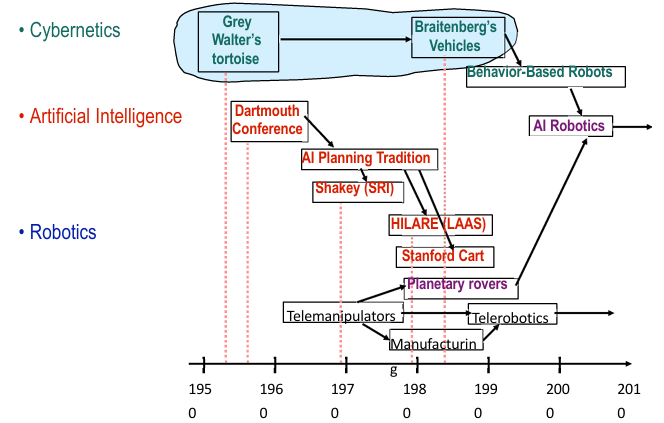
\includegraphics[scale=0.7]{1.precursori robotica moderna.png}
        \caption{The three historical branches of robotics}
        \captionsetup{font=footnotesize}
    \end{figure}

\textbf{The cybernetic branch.} It begins with Grey Walter's \textit{Tortoise} (1953), an extremely simple robot (two sensors, two reflex behaviors) that already displays complex, emergent behavior governed by \textbf{negative feedback} (the system continuously compares its state to a reference and self-regulates). Braitenberg later formalizes this idea with his \textit{Vehicles}: apparently intentional behaviors (fear, aggression, love) can emerge from simple sensor-motor wiring, with no internal world model at all.

\textbf{The AI/symbolic branch.} Originating from the Dartmouth Conference (1956), it culminates in \textit{Shakey} (SRI, 1966), the first robot to physically implement the \textbf{Sense $\rightarrow$ Plan $\rightarrow$ Act} cycle using the STRIPS planner. It works well, but only in structured, simplified environments (rooms with colored geometric objects).

\textbf{The turning point.} Rodney Brooks (MIT, 1987) sharply criticizes the symbolic approach ("Elephants don't play chess") and proposes \textbf{behavior-based / reactive robotics}: no planning, no world model, only direct sensor-actuator relations.

The \textit{Roomba} shows this approach works in practice: a purely reactive robot, with no map and no planning, can perform a real-world task (cleaning) effectively and cheaply.

\begin{defbox}{Key Theoretical Opposition}
    \begin{itemize}
\item \textbf{Hierarchical approach}: relies on an internal world model and explicit planning before acting. Accurate but computationally expensive and dependent on structured environments.

\item \textbf{Reactive approach}: relies on direct sensor-actuator coupling with no internal representation . Fast, cheap, and robust, but unable to handle long-term goals or complex reasoning.


    \end{itemize}
\end{defbox}

This opposition is the conceptual thread connecting the historical introduction to the formal \textbf{Hierarchical}, \textbf{Reactive}, and \textbf{Hybrid} control paradigms covered in the rest of the chapter.

\subsection{Robot Control Architectures: Foundations}

% ============================================================
% SLIDE 12 — Architetture (general diagram)
% ============================================================
\subsubsection{Architectures: General Diagram}

This chapter introduces the general schematic that will be used  to describe any robot control architecture. The diagram shows the robot as a closed loop with the \textbf{World}:

\begin{itemize}
    \item The \textbf{World} sends data to a \textbf{Sensor} module.
    \item The \textbf{Sensor} module feeds information into the \textbf{Robot Control System}, which is composed of multiple parallel \textbf{Behaviors} (Behavior 1, Behavior 2, Behavior 3, \ldots).
    \item The outputs of the behaviors are combined/arbitrated (represented by the small circular nodes) into a single command stream.
    \item This command stream is sent to the \textbf{Actuator} module, which finally acts back on the \textbf{World}, closing the loop.
\end{itemize}

    \begin{figure}[H]
        \centering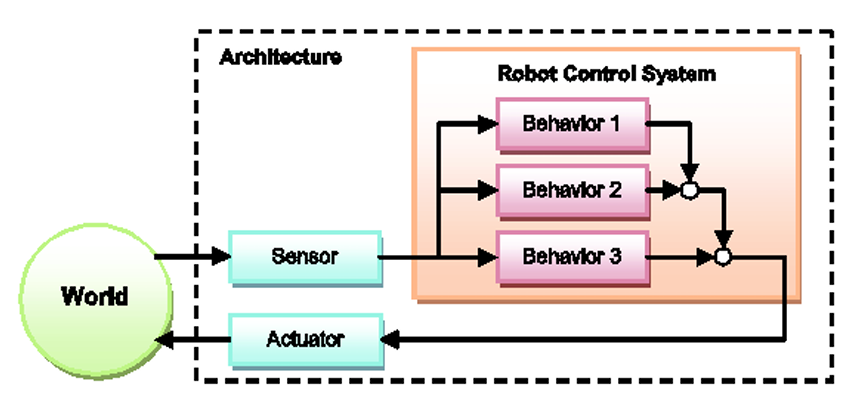
\includegraphics[scale=0.7]{2.robot_architecture.png}
        \caption{General Robot Architecture}
        \captionsetup{font=footnotesize}
    \end{figure}

\begin{defbox}{Robot Architecture (informal, diagrammatic view)}
A robot architecture is the overall organization of the software (and, indirectly, hardware) that connects sensing, decision-making (behaviors), and actuation into a coherent control loop with the environment..
\end{defbox}

 Different architectural paradigms (Hierarchical, Reactive, Hybrid, covered later in this chapter) differ mainly in \textit{how} the \texttt{Behavior} block(s) inside the \texttt{Robot Control System} are organized and combined


% ============================================================
% SLIDE 14 — Organizzazione del software
% ============================================================
\subsubsection{Software Organization}

This chapter provides the formal definition of \textit{Architecture}

\begin{defbox}{Architecture (Software Organization)}
The overall style of design and organization of software is called an \textbf{Architecture}. It can be characterized in (at least) two complementary ways:
\begin{itemize}
    \item It provides a way of organizing a control system. In addition, it provides a structure and imposes constraints on how control problems are solved \textbf{[Mataric]}.
    \item It describes a set of architectural components and how they interact with each other \textbf{[Dean \& Wellman]}.
\end{itemize}
\end{defbox}

These two definitions highlight two complementary aspects of the same concept. Both views will be used implicitly when we later describe the Hierarchical, Reactive, and Hybrid paradigms: each paradigm is a different \textit{architecture} in exactly this sense: a different set of constraints on how Sense, Plan, and Act components are structured and connected.

% ============================================================
% SLIDE 15 — Tipi di Architetture [Lewis]
% ============================================================
\subsubsection{ Types of Architectures}

Lewis proposes a three-level classification of what "architecture" can mean, depending on the level of abstraction being described.

\begin{itemize}
\item \textbf{Operational Architecture}.
Describes \textbf{what} the system does at a high level, \textbf{not how} it does it.


\item \textbf{System Architecture}.
Describes \textbf{how} a system works in terms of its \textbf{main subsystems} and their organization.

\item \textbf{Technical Architecture}.
Describes \textbf{how} a system works in terms of \textbf{implementation details}, such as the programming language, data structures, and low-level design choices.

\end{itemize}



% ============================================================
% SLIDE 16 — Good Software Engineering
% ============================================================
\subsubsection{Good Software Engineering Principles}

The three classical software engineering principles that a good robot control architecture should satisfy.

\begin{itemize}
\item \textbf{Abstraction}.
Ignoring irrelevant implementation details allows one to reason about the general organization of a system. This is typically expressed through a \textbf{semiformal description} (e.g., block diagrams such as the Sense-Plan-Act schema) rather than through full formal specification or actual code.


\item \textbf{Modularity}.
A design property characterized by:
\begin{itemize}
    \item \textbf{High cohesion}: the possibility of substituting different algorithms within the same module to produce the same type of results.

    \vspace{0.2cm}
    \item \textbf{Low coupling}: minimal dependencies between different modules, so that changes in one module have limited impact on others;

    \vspace{0.2cm}
    \item \textbf{Support for testing}: modules can be tested independently, which simplifies verification and debugging.
\end{itemize}


\item \textbf{Generality}.
The principle of \textbf{not reinventing anything}: whenever possible, existing, well-tested algorithms, components, or design patterns should be reused rather than redesigned from scratch.
\end{itemize}

\subsection{Robot Control Paradigms}

% ============================================================
% SLIDE 17 — I paradigmi per il controllo dei robot (intro)
% ============================================================
\subsubsection{Introduction to Robot Control Paradigms}

We introduces the three classical paradigms that will structure the rest of the chapter, framing them with an important epistemological caveat.

\begin{itemize}
    \item \textbf{No paradigm has absolute validity}: some problems are better addressed with certain paradigms rather than others.
    \item Choosing the \textbf{right paradigm} for a given problem often makes it much easier to reach the best possible solution.
    \item \textbf{Traditionally}, three paradigms are identified:
    \begin{itemize}
        \item \textbf{Hierarchical}
        \item \textbf{Reactive}
        \item \textbf{Hybrid}
    \end{itemize}
\end{itemize}

\begin{defbox}{Control Paradigm}
A control paradigm is a general philosophy (an \textit{operational architecture}) for organizing how a robot senses, decides, and acts. It is not tied to a specific algorithm or implementation, but defines the overall relationship between perception, reasoning, and action.
\end{defbox}



% ============================================================
% SLIDE 18 — Robot primitives: SENSE, PLAN, ACT
% ============================================================
\subsubsection{Robot Primitive Functions}

 The criterion that will be used to distinguish the three paradigms: they differ in \textbf{how the main primitive functions of a robot are organized}, not in \textit{which} functions exist, but in how they are connected and sequenced.

\begin{defbox}{Robot Primitive Functions}
Every robot control system, regardless of paradigm, is built from three primitive functions:
\begin{itemize}
    \item \textbf{Perception (SENSE)}: acquiring and interpreting information about the environment;
    \item \textbf{Planning (PLAN)}: deciding what to do, based on available information;
    \item \textbf{Action/Actuation (ACT)}: executing commands through the robot's actuators.
\end{itemize}
\end{defbox}

This is a crucial conceptual step: it reduces the apparent complexity of comparing different architectures to a single question: \textit{"How are SENSE, PLAN, and ACT connected to one another?"} As we will see:
\begin{itemize}
    \item the \textbf{Hierarchical} paradigm connects them sequentially ($S \rightarrow P \rightarrow A$);
    \item the \textbf{Reactive} paradigm removes PLAN almost entirely, connecting SENSE directly to ACT ($S \rightarrow A$);
    \item the \textbf{Hybrid} paradigm keeps PLAN as a separate, higher-level module, while SENSE and ACT are tightly coupled at a lower level ($P$, $S \rightarrow A$).
\end{itemize}







\subsection{The Hierarchical Paradigm}

% ============================================================
% SLIDE 21 — Paradigms overview (S-P-A, S-A, P,S-A)
% ============================================================
\subsubsection{Robot Control Paradigms: Notation Overview}

This chapter introduces the compact notation that will be used to distinguish the three paradigms, based on how SENSE (S), PLAN (P), and ACT (A) are connected:

\begin{itemize}
    \item \textbf{Hierarchical: S-P-A}: sequential flow from Sense to Plan to Act.
    \item \textbf{Reactive: S-A}: Sense connects directly to Act, bypassing Plan.
    \item \textbf{Hybrid: P, S-A}: Plan exists as a separate module, while Sense and Act are tightly coupled.
\end{itemize}

\begin{center}
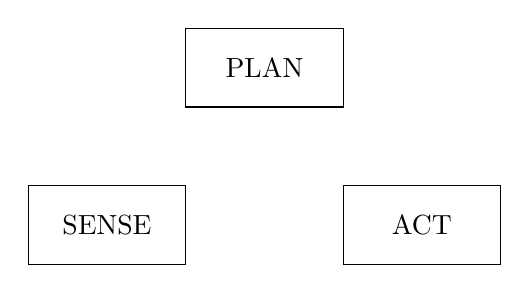
\begin{tikzpicture}[node distance=2cm, box/.style={draw, minimum width=2cm, minimum height=1cm}]
    \node[box] (plan) at (2,2) {PLAN};
    \node[box] (sense) at (0,0) {SENSE};
    \node[box] (act) at (4,0) {ACT};
\end{tikzpicture}
\end{center}

 Note that at this stage the three boxes are still \textbf{unconnected}. this chapter only introduces the shorthand notation ($S$-$P$-$A$, $S$-$A$, $P,S$-$A$) that will be visually instantiated with actual arrows in the following, starting with the Hierarchical paradigm.

% ============================================================
% SLIDE 22 — Il Paradigma Gerarchico (S-P-A diagram)
% ============================================================
\subsubsection{The Hierarchical Paradigm: S-P-A}

This slide gives the first fully-connected diagram: the \textbf{Hierarchical} paradigm, denoted \textbf{S-P-A}.

\begin{center}
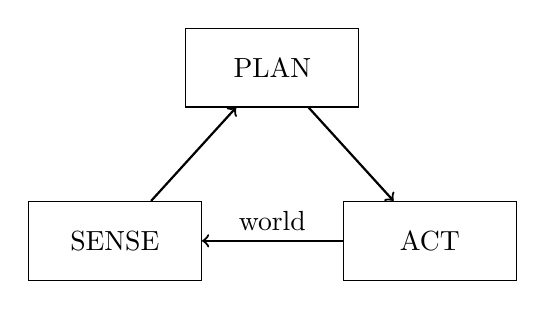
\begin{tikzpicture}[node distance=2.5cm, box/.style={draw, minimum width=2.2cm, minimum height=1cm}]
    \node[box] (plan) at (2,2.2) {PLAN};
    \node[box] (sense) at (0,0) {SENSE};
    \node[box] (act) at (4,0) {ACT};

    \draw[->, thick] (sense) -- (plan);
    \draw[->, thick] (plan) -- (act);
    \draw[<-, thick] (sense) -- (act) node[midway, above] {world};
\end{tikzpicture}
\end{center}

\begin{defbox}{Hierarchical Paradigm (S-P-A)}
A control paradigm in which information flows \textbf{sequentially}: SENSE processes raw sensor data into sensed information, which is passed to PLAN; PLAN reasons over this information (possibly combined with an internal world model) and produces directives; ACT translates these directives into actuator commands, which affect the world; the world is then perceived again by SENSE, closing the loop.
\end{defbox}



% ============================================================
% SLIDE 23 — Table Input/Output for Hierarchical paradigm
% ============================================================


We can specializes the general primitives table to the Hierarchical paradigm, explicitly showing the sequential data flow via arrows between rows.

\begin{center}
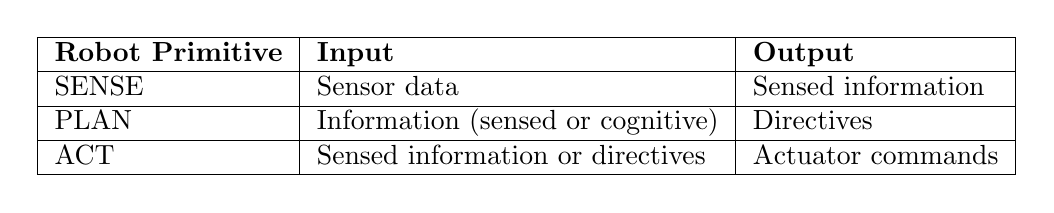
\begin{tikzpicture}[node distance=1.5cm]
    \node (t) {
    \begin{tabular}{|l|l|l|}
    \hline
    \textbf{Robot Primitive} & \textbf{Input} & \textbf{Output} \\
    \hline
    SENSE & Sensor data & Sensed information \\
    \hline
    PLAN & Information (sensed or cognitive) & Directives \\
    \hline
    ACT & Sensed information or directives & Actuator commands \\
    \hline
    \end{tabular}
    };
\end{tikzpicture}
\end{center}

The key distinguishing feature of the Hierarchical paradigm  is that here \textbf{ACT's input is specifically the \textit{directives} coming from PLAN}, not sensed information directly. This confirms the strict $SENSE \rightarrow PLAN \rightarrow ACT$ sequence shown in the previous diagram: every action is mediated by a planning step, with no shortcut from perception to action.

% ============================================================
% SLIDE 24 — Gerarchico: AI Classico (cognition role)
% ============================================================
\subsubsection{ Hierarchical: Classical AI - The Role of Cognition}

\begin{itemize}
    \item \textbf{Cognition} is used to interpret perception and to plan the actions of the actuators.
    \item The \textbf{perception module} generates a description of the world, which is used by the \textbf{cognition module} to produce a sequence of actions for the \textbf{action module}.
\end{itemize}

\begin{defbox}{Cognition (in the Hierarchical - Classical AI sense)}
The symbolic reasoning process that takes as input a description of the world (produced by perception) and produces, as output, a sequence of actions intended to achieve a given goal. Cognition is the "PLAN" primitive instantiated with explicit, symbolic reasoning over an internal world description.
\end{defbox}

This chapter makes explicit \textit{why} PLAN needs an intermediate representation: cognition cannot reason directly over raw sensor data (e.g., pixel values), it needs perception to first abstract that data into a symbolic \textit{description of the world} it can reason about. 
% ============================================================
% SLIDE 25 — Gerarchico: AI Classico (world model)
% ============================================================


\begin{itemize}
    \item In hierarchical architectures, \textbf{perception} is used to establish and maintain a correspondence between the \textbf{internal model of the world} (or map) and the \textbf{external world}.
    \item Typically, the world model contains:
    \begin{itemize}
        \item an \textbf{a priori} representation of the environment in which the robot operates;
        \item the \textbf{perceived sensory information};
        \item other information necessary for \textbf{task execution}.
    \end{itemize}
    \item The world representation is \textbf{updated every time} the robot perceives the environment, and the action plan is established \textbf{based on this representation}.
\end{itemize}

\begin{defbox}{World Model (Internal Map/Knowledge Base)}
An internal, symbolic representation of the environment maintained by the robot, combining a-priori knowledge, real-time sensory data, and task-relevant information. Planning decisions are made with respect to this model rather than directly on raw sensor input.
\end{defbox}

This is the central structural weakness that the \textbf{Reactive paradigm}  will explicitly reject: maintaining an accurate, up-to-date world model is computationally expensive and fragile in unstructured or dynamic environments. This is exactly the criticism raised by Brooks, who instead claimed "the world is the best model of itself."

% ============================================================
% SLIDE 26 — Gerarchico: AI Classico (functional decomposition diagram)
% ============================================================
\subsubsection{ Hierarchical: Classical AI - Functional Task Decomposition}

\begin{itemize}
    \item \textbf{Logical and functional} subdivision and distribution of tasks.
    \item \textbf{Horizontal and sequential} subdivision of the information chain processed by the centralized system.
\end{itemize}

\begin{center}
\begin{tikzpicture}[node distance=0cm, box/.style={draw, minimum width=1.8cm, minimum height=2.5cm, align=center}]
    \node[box] (perc) {Perception};
    \node[box, right=0cm of perc] (model) {Modelling};
    \node[box, right=0cm of model] (plan) {Planning};
    \node[box, right=0cm of plan] (exec) {Execution};
    \node[box, right=0cm of exec] (motor) {Motor Control};

    \node[left=1cm of perc] (sensors) {Sensors};
    \node[right=1cm of motor] (actuators) {Actuators};

    \draw[->, thick] (sensors) -- (perc);
    \draw[->, thick] (motor) -- (actuators);
\end{tikzpicture}
\end{center}

\begin{defbox}{Functional Pipeline (Classical AI)}
A strictly sequential chain of specialized modules --- \textit{Perception $\rightarrow$ Modelling $\rightarrow$ Planning $\rightarrow$ Execution $\rightarrow$ Motor Control} --- where each module processes the output of the previous one and passes its result to the next, from raw sensor data all the way to actuator commands.
\end{defbox}

 This is the detailed, five-module refinement of the simple three-box S-P-A diagram: \textit{Perception} and \textit{Modelling} together implement SENSE (raw data $\rightarrow$ world model), \textit{Planning} implements PLAN, and \textit{Execution} + \textit{Motor Control} together implement ACT (directives $\rightarrow$ actuator commands). This finer decomposition is an example of the \textbf{modularity} principle.

% ============================================================
% SLIDE 27 — Gerarchico: AI Classico (three planner levels)
% ============================================================
\subsubsection{ Hierarchical: Classical AI - The Three-Level Planner}

Generally, the Planner module is structured into three levels:

\begin{itemize}
\item \textbf{Strategic Level}
The highest level of the planner: generates a \textbf{strategy} based on the overall task the robot must perform (answers \textit{"what should the robot do?"}).
\item \textbf{Tactical Level}
The intermediate level: generates \textbf{commands} by interpreting instructions coming from the strategic level (answers \textit{"how should tasks be executed?"}).


\item \textbf{Executive Level}
The lowest level: receives macro-commands generated by the tactical level and handles \textbf{real-time control} of the actuators (answers \textit{"how are commands actually executed?"}).
\end{itemize}


\begin{center}
\begin{tikzpicture}[
    node distance=0.9cm,
    box/.style={draw, minimum width=6cm, minimum height=1cm, align=center, font=\footnotesize, text width=5.6cm}
]
    \node[box] (strat) {\textbf{Strategic}\\ This level generates goals and strategies for achieving those goals which result in the achievement of an overall objective};
    \node[box, below=of strat] (tact) {\textbf{Tactical}\\ This level generates the tactics by which a goal is to be achieved};
    \node[box, below=of tact] (exec) {\textbf{Executive}\\ This level executes the tactical plan};

    \draw[<->, thick] (strat) -- (tact);
    \draw[<->, thick] (tact) -- (exec);

    \node[right=0.2cm of strat, text width=2cm, font=\footnotesize] {What the robot must do};
    \node[right=0.2cm of tact, text width=2cm, font=\footnotesize] {How to execute tasks};
    \node[right=0.2cm of exec, text width=2cm, font=\footnotesize] {Command execution};
\end{tikzpicture}
\end{center}



 The bidirectional arrows between levels are important: information does not flow only top-down (goals $\rightarrow$ commands); there is also bottom-up feedback (e.g., execution failures or sensed obstacles reported back to the tactical/strategic levels), which allows some degree of re-planning. 
 
 This three-level structure is a refinement of the single "PLAN" box, and it is exactly what the \textbf{Nested Hierarchical Controller} will instantiate concretely as Mission Planner / Navigator / Pilot.

% ============================================================
% SLIDE 28 — Gerarchico: AI Classico (worked example)
% ============================================================
\subsubsection{ Hierarchical: Classical AI - Worked Example}

\textbf{Example.} Task: \textit{"get the bottle from the fridge"} (\textit{"prendi la bottiglia dal frigorifero"}).

\begin{itemize}
    \item \texttt{Strategic Level}: go to the kitchen, go in front of the fridge, open the fridge, take the bottle\ldots

    \vspace{0.2cm}
    \item \texttt{Tactical Level}:
    \begin{itemize}
        \item Go to the kitchen: \texttt{move\_base(X1,Y1); move\_base(X2,Y2)}\ldots
        \item Open the fridge: \texttt{move\_arm(P1), Open\_Hand()}\ldots
    \end{itemize}

    \vspace{0.2cm}
    \item \texttt{Executive Level}: \texttt{move\_base(X1,Y1); move\_base(X2,Y2); move\_arm(P1)}\ldots
\end{itemize}

 This example makes the three-level hierarchy concrete: the strategic level reasons in terms of high-level sub-goals (natural-language-like instructions), the tactical level translates each sub-goal into a sequence of parametrized robot function calls, and the executive level is what actually gets sent, in real time, to the low-level motor controllers. Notice how the level of abstraction decreases monotonically from top to bottom — this is a direct illustration of the \textbf{abstraction} principle from Slide 16.

% ============================================================
% SLIDE 29 — Nested Hierarchical Controller
% ============================================================
\subsubsection{ The Nested Hierarchical Controller (NHC)}

This chapter presents a concrete instantiation of the hierarchical paradigm: the \textbf{Nested Hierarchical Controller (NHC)}, structured as SENSE / PLAN / ACT, where PLAN itself is subdivided into three nested modules:

\begin{itemize}
    \item The \textbf{Mission Planner} module receives a mission from a human operator (e.g., "get the box in the next room") and encodes it into terms understandable by the other modules; it also retrieves the robot's position and goal from the map.

    \vspace{0.2cm}
    \item The \textbf{Navigator} module receives this information and generates a path (trajectory) from the current position to the goal.

    \vspace{0.2cm}
    \item The \textbf{Pilot} module determines the actions that the actuators must perform in order to follow the planned path.
\end{itemize}

\begin{center}
\begin{tikzpicture}[node distance=0.6cm, box/.style={draw, minimum width=2.6cm, minimum height=0.9cm, align=center}]
    \node[box, minimum height=5cm, minimum width=2.2cm] (wm) {World Model / \\ Knowledge Base};

    \node[box, right=1.5cm of wm, yshift=1.8cm] (mp) {Mission Planner};
    \node[box, below=0.3cm of mp] (nav) {Navigator};
    \node[box, below=0.3cm of nav] (pilot) {Pilot};

    \node[box, below=0.3cm of pilot, minimum width=2.6cm] (llc) {Low-level Controller};

    \node[below=0.6cm of llc, xshift=-0.8cm] (drive) {drive};
    \node[below=0.6cm of llc, xshift=0.8cm] (steer) {steer};

    \node[below=0.6cm of wm] (sensors) {sensors};

    \draw[<->, thick] (wm) -- (mp);
    \draw[<->, thick] (wm) -- (nav);
    \draw[<->, thick] (wm) -- (pilot);
    \draw[<->, thick] (pilot) -- (llc);
    \draw[->, thick] (llc.south west) -- (drive);
    \draw[->, thick] (llc.south east) -- (steer);
    \draw[->, thick] (sensors) -- (wm);

    \node[left=0.1cm of wm, yshift=1.5cm, rotate=90] {\footnotesize SENSE};
    \node[right=3.2cm of wm, yshift=1.5cm] {\footnotesize PLAN};
    \node[right=3.2cm of wm, yshift=-2.5cm] {\footnotesize ACT};
\end{tikzpicture}
\end{center}




\begin{defbox}{Nested Hierarchical Controller (NHC)}
A hierarchical architecture in which the PLAN module is internally organized as a nested chain of increasingly detailed planners --- \textbf{Mission Planner} (mission $\rightarrow$ goal) $\rightarrow$ \textbf{Navigator} (goal $\rightarrow$ path) $\rightarrow$ \textbf{Pilot} (path $\rightarrow$ path subsegment/actuator directives) --- all of which read from and write to a shared \textbf{World Model / Knowledge Base}.
\end{defbox}


% ============================================================
% SLIDE 30 — Architetture Gerarchiche (common characteristics)
% ============================================================
\subsubsection{ Hierarchical Architectures: Common Characteristics}


\begin{itemize}
    \item \textbf{Hierarchical structure};
    \item \textbf{Clear division} of functionalities;
    \item \textbf{Predetermined} communication and control patterns;
    \item \textbf{Higher levels provide sub-goals} for lower levels;
    \item \textbf{Requires a symbolic representation} of the world.
\end{itemize}

 These architectures are \textbf{appropriate for structured and predictable environments}.


